% Generated captions for the corrected rebuild.
\section*{Figures}

\begin{center}
\begin{minipage}{\linewidth}
\captionsetup{type=figure,hypcap=false}
\centering
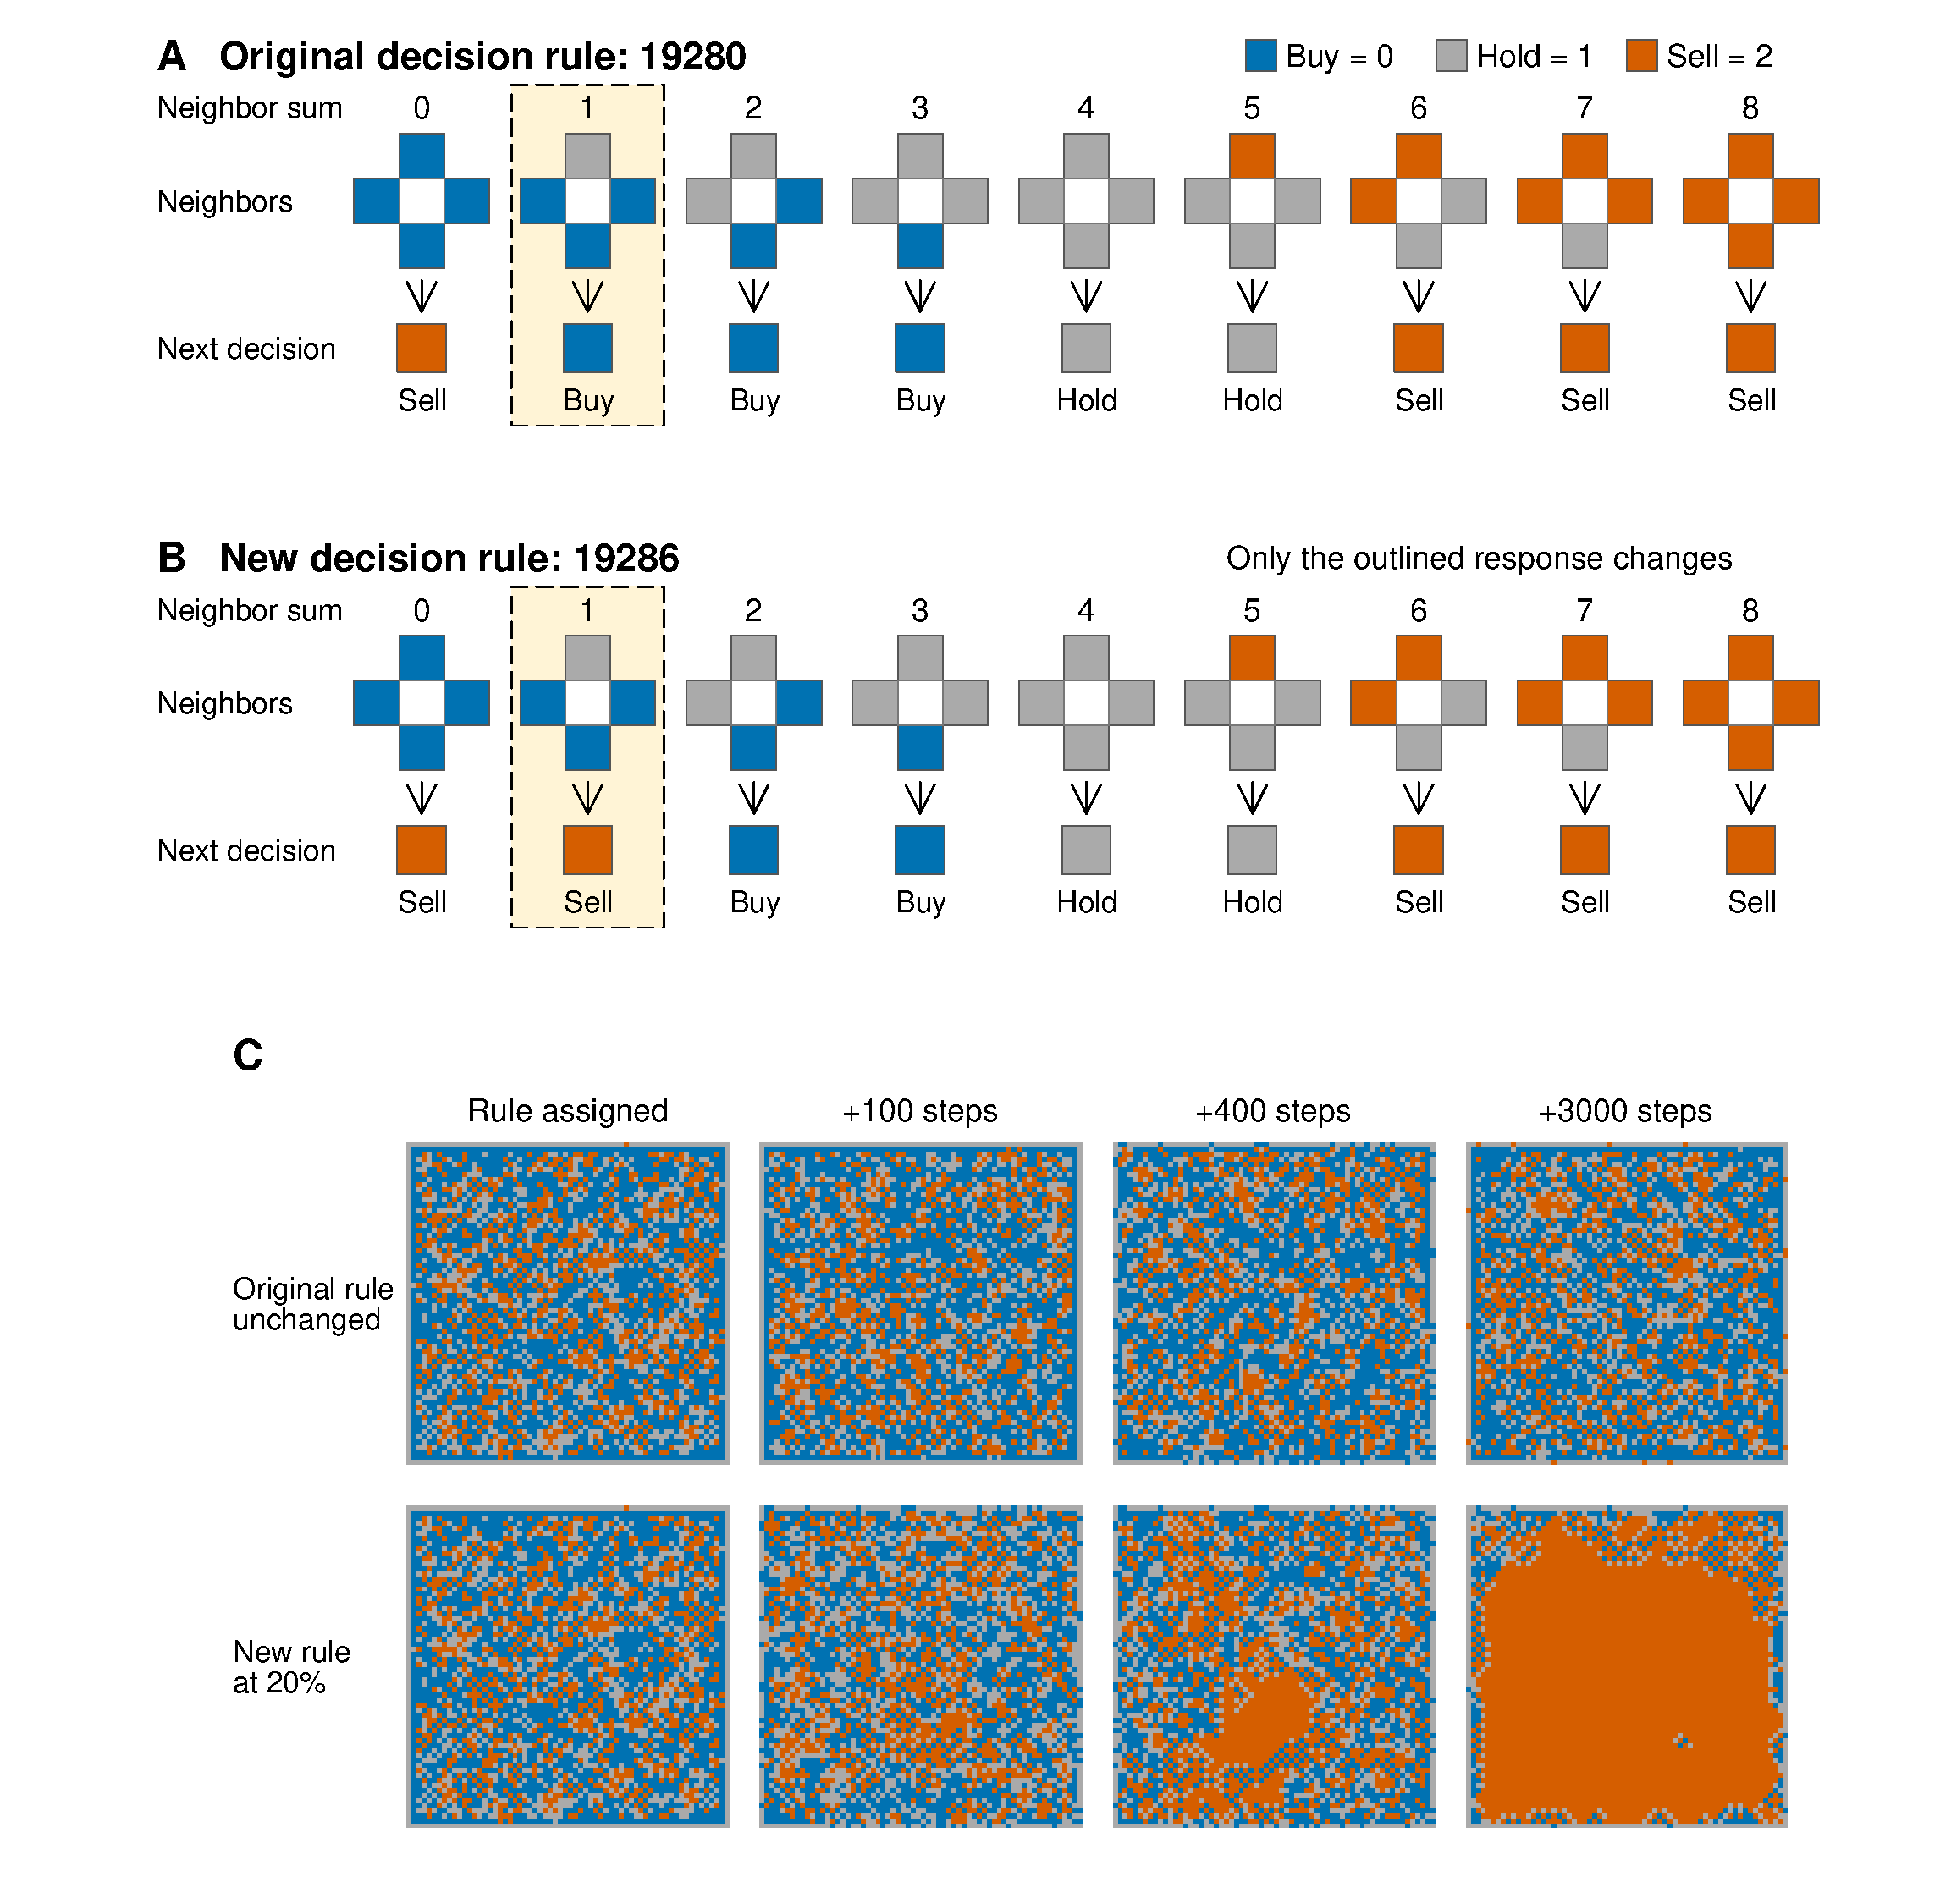
\includegraphics[width=0.95\linewidth]{figs/Fig1-RuleQuench.pdf}
\caption{The changed response and paired market decisions.
\textbf{(A)}~Baseline Rule~19280. \textbf{(B)}~Activated Rule~19286.
Each cross contains the four neighbors used to determine the next decision,
shown below its arrow. The hollow center is the trader being updated;
its current decision does not enter the lookup table. Blue, gray, and
orange denote Buy~(0), Hold~(1), and Sell~(2). One arrangement represents
each neighbor sum; every arrangement with that sum produces the same
response. The outlined column is the only rule change: three Buys and
one Hold produce Buy under the baseline and Sell under activation.
\textbf{(C)}~Paired $64\times64$ grids at activation and after 100,
400, and 3,000 steps. The upper row retains the baseline rule; the lower
assigns the new rule to 20\% of interior traders. Both paths share a
1,000-step baseline, $h=100$, and active technical traders. Starting
market 14 was selected from 50 by proximity to the
median paired difference in peak Sell fraction. Ensemble outcomes and
conditional onset times appear in Supplementary Table~\ref{tab:paired-switch}.}
\label{fig:rule-quench}
\end{minipage}
\end{center}

\clearpage

\begin{center}
\begin{minipage}{\linewidth}
\captionsetup{type=figure,hypcap=false}
\centering
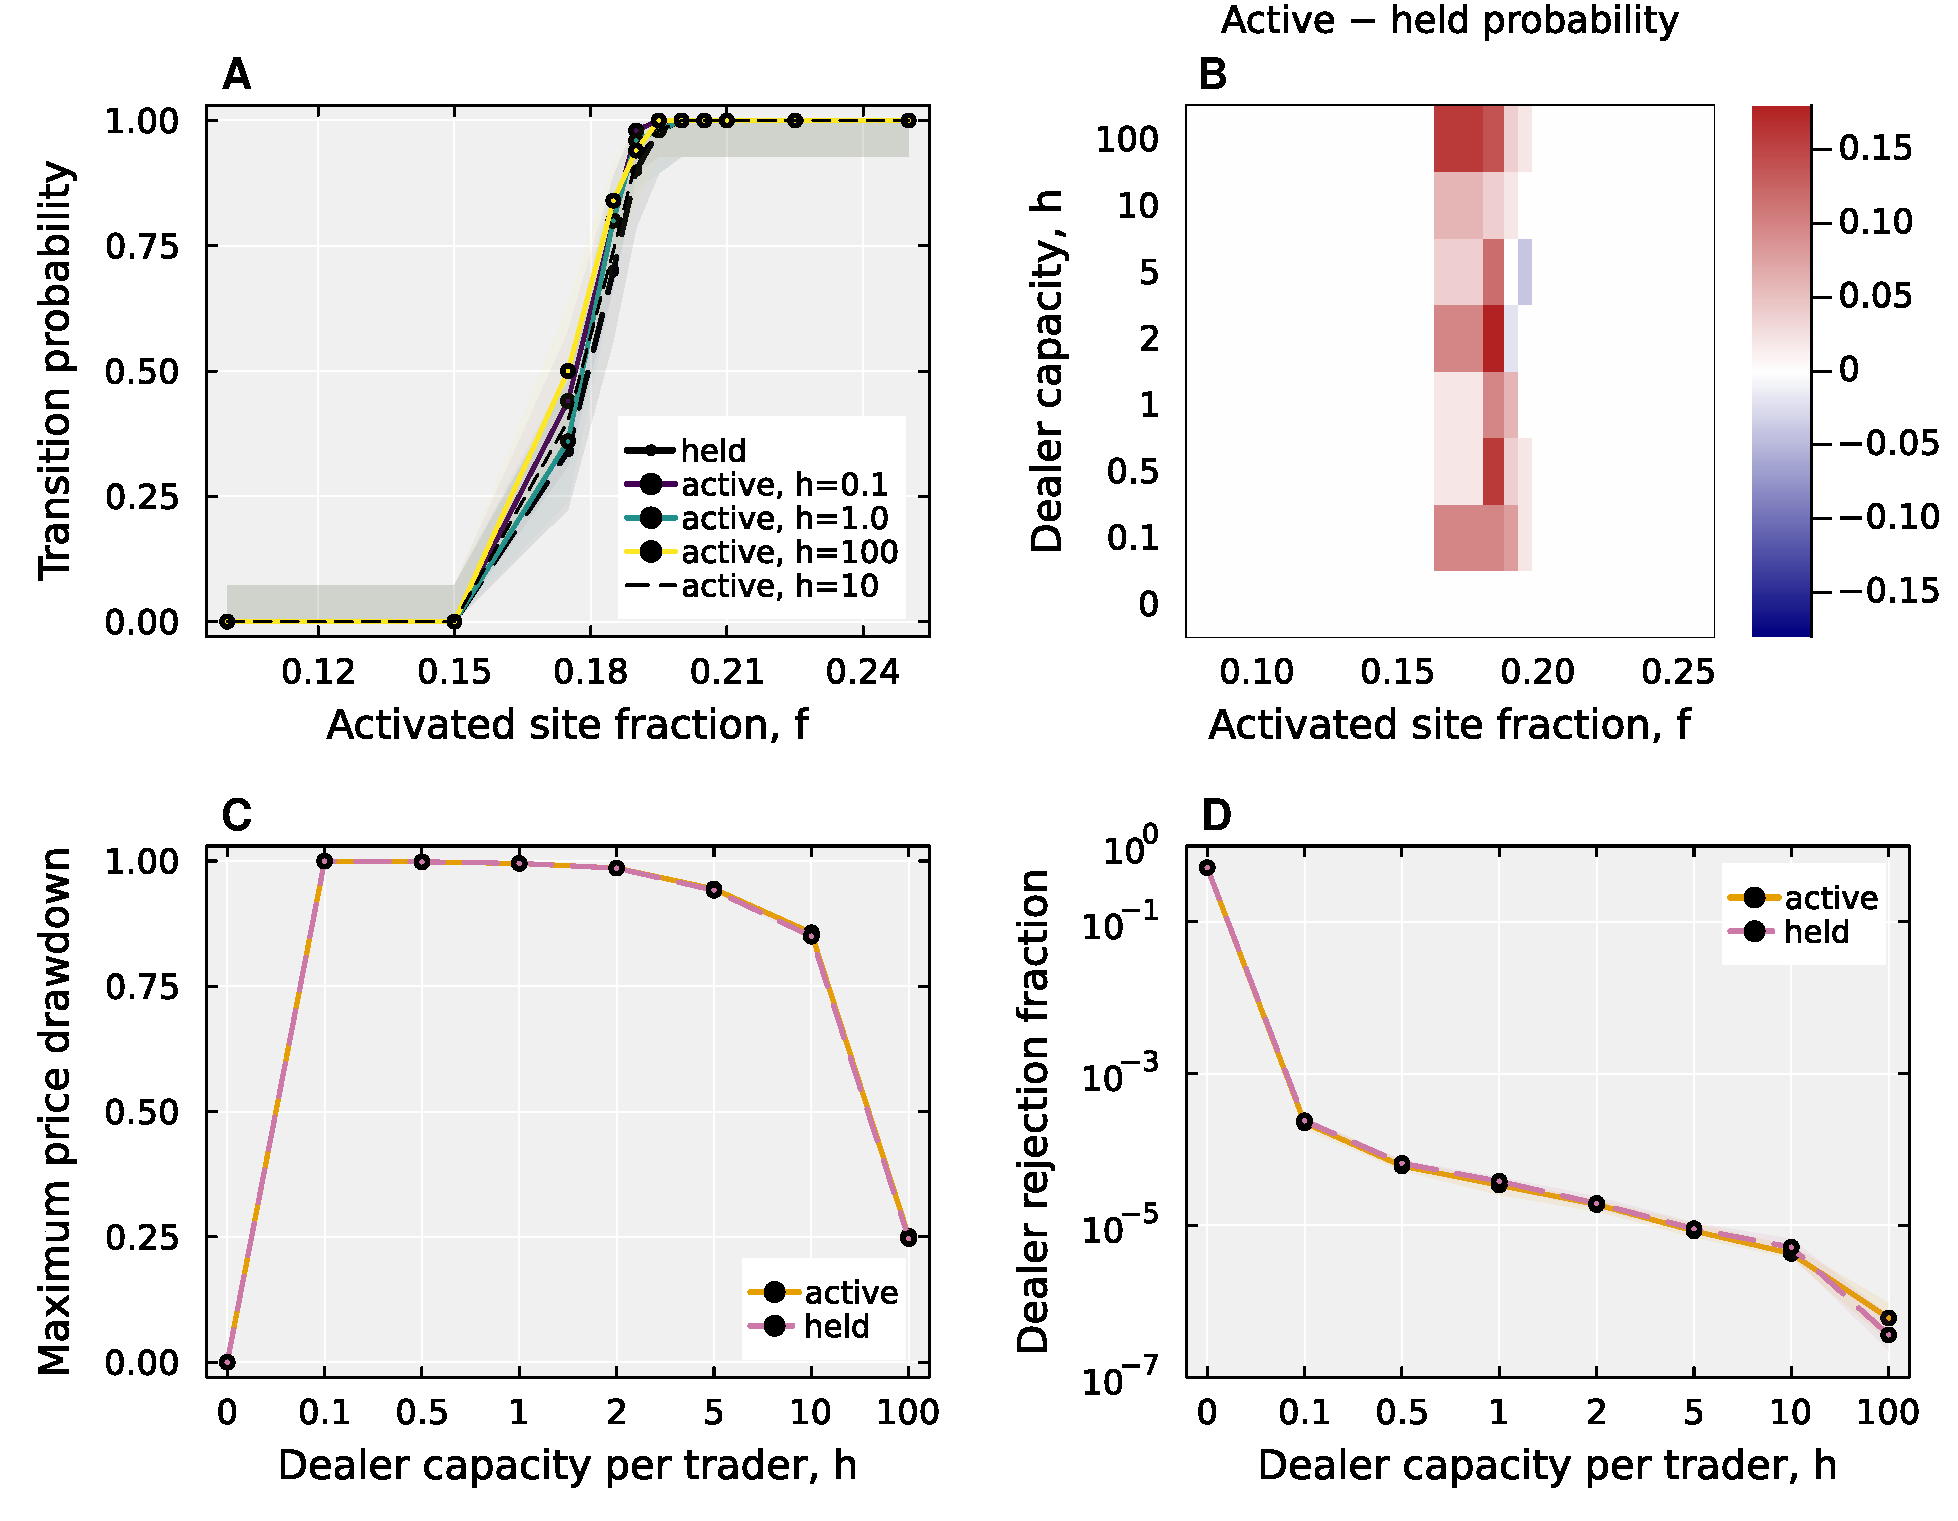
\includegraphics[width=0.97\linewidth]{figs/Fig2-ReservoirQuench.pdf}
\caption{Rule changes across dealer reserve depths over 3,000 post-switch steps.
\textbf{(A)}~Probability of an interior Sell majority with technical
traders held or active. Bands are 95\% Wilson intervals over 50 starting
markets. \textbf{(B)}~Active-minus-held majority probability at each
depth and target fraction. \textbf{(C)}~Median maximum drawdown at
$f=0.20$, with interquartile bands. \textbf{(D)}~Median fraction of
post-switch eligible orders rejected at $f=0.20$, on a logarithmic
axis with interquartile bands. Depth $h$ is initial dealer shares per trader and also determines
price sensitivity through the reserve curve. The $h=10$ dashed overlay
in A is a distinct finite-depth comparison; the deep arm is $h=100$.
At zero depth only opposing trader orders match and price stays fixed.
Panels C and D describe switched markets. Matched no-switch drawdowns
and paired differences appear in Supplementary Table~\ref{tab:paired-switch}.}
\label{fig:reservoir}
\end{minipage}
\end{center}

\clearpage

\begin{center}
\begin{minipage}{\linewidth}
\captionsetup{type=figure,hypcap=false}
\centering
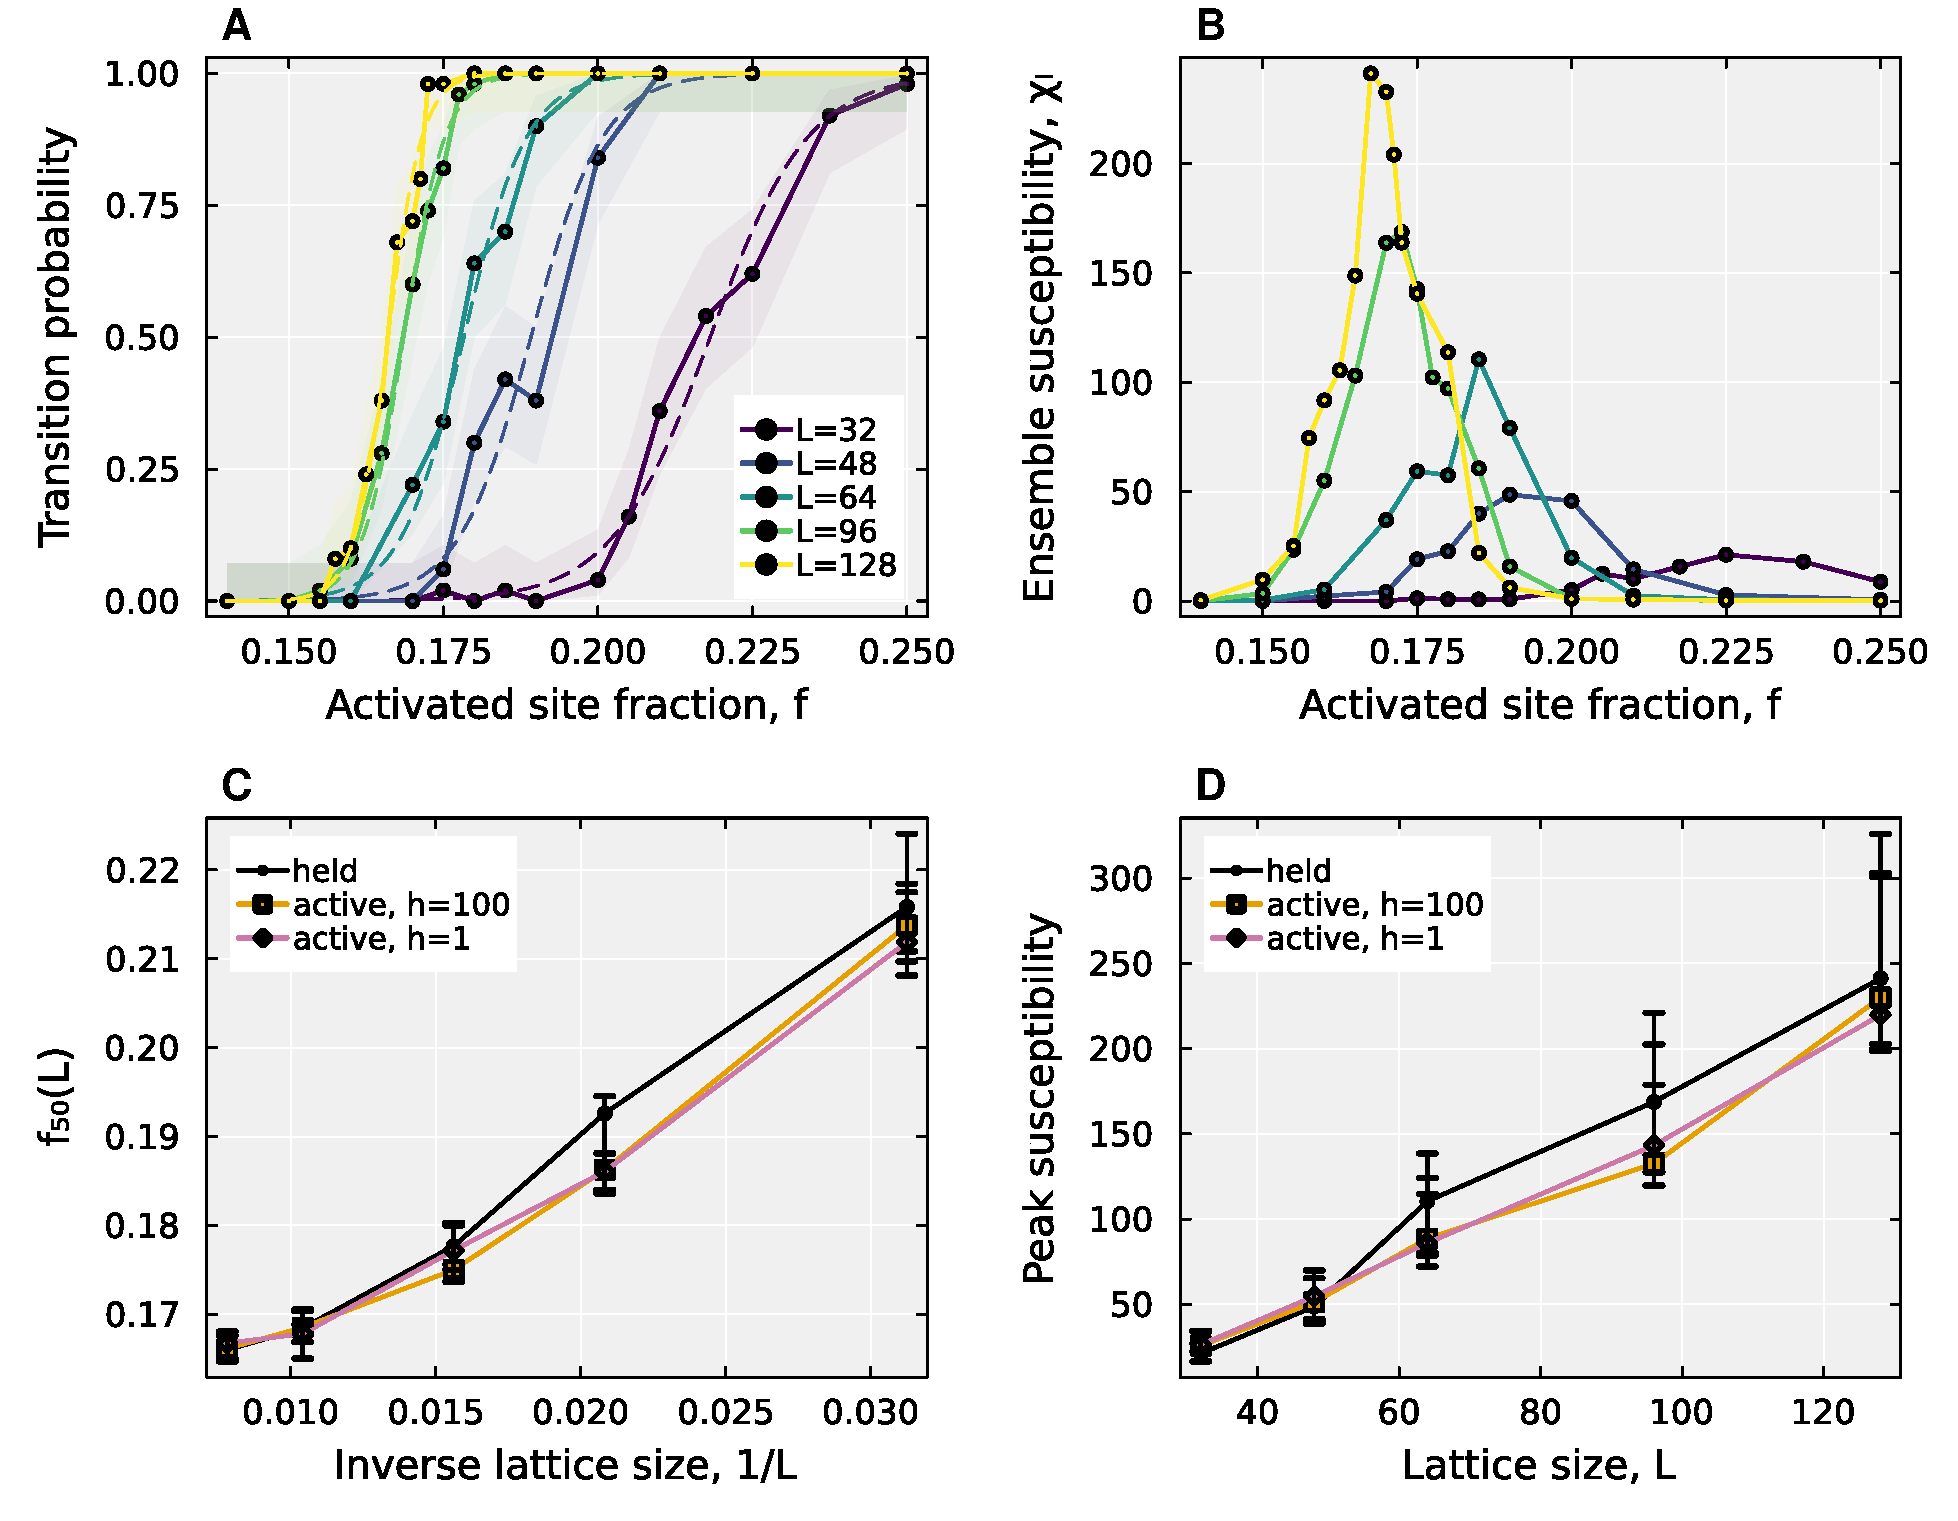
\includegraphics[width=0.97\linewidth]{figs/Fig3-FiniteSizeQuench.pdf}
\caption{Market size and the formation of a Sell majority
over 50 starting markets and 3,000 post-switch steps. \textbf{(A)}~Majority probability with technical
traders held, with 95\% Wilson bands. \textbf{(B)}~Susceptibility with
technical traders held: the variance across markets of the final
500-step mean Sell fraction, multiplied by the number of interior traders.
\textbf{(C)}~Interpolated fraction $f_{50}(L)$ at which half the markets
reached a majority, against inverse grid size, for held traders at $h=100$ and active traders at
$h=1$ and $h=100$. \textbf{(D)}~Sampled maximum susceptibility versus
grid size. Error bars in C and D are 95\% whole-market bootstrap
intervals. Solid lines connect tested values; dashed curves in A are
logistic fits. No law for indefinitely large grids was fitted.}
\label{fig:finite-size}
\end{minipage}
\end{center}

\clearpage

\begin{center}
\begin{minipage}{\linewidth}
\captionsetup{type=figure,hypcap=false}
\centering
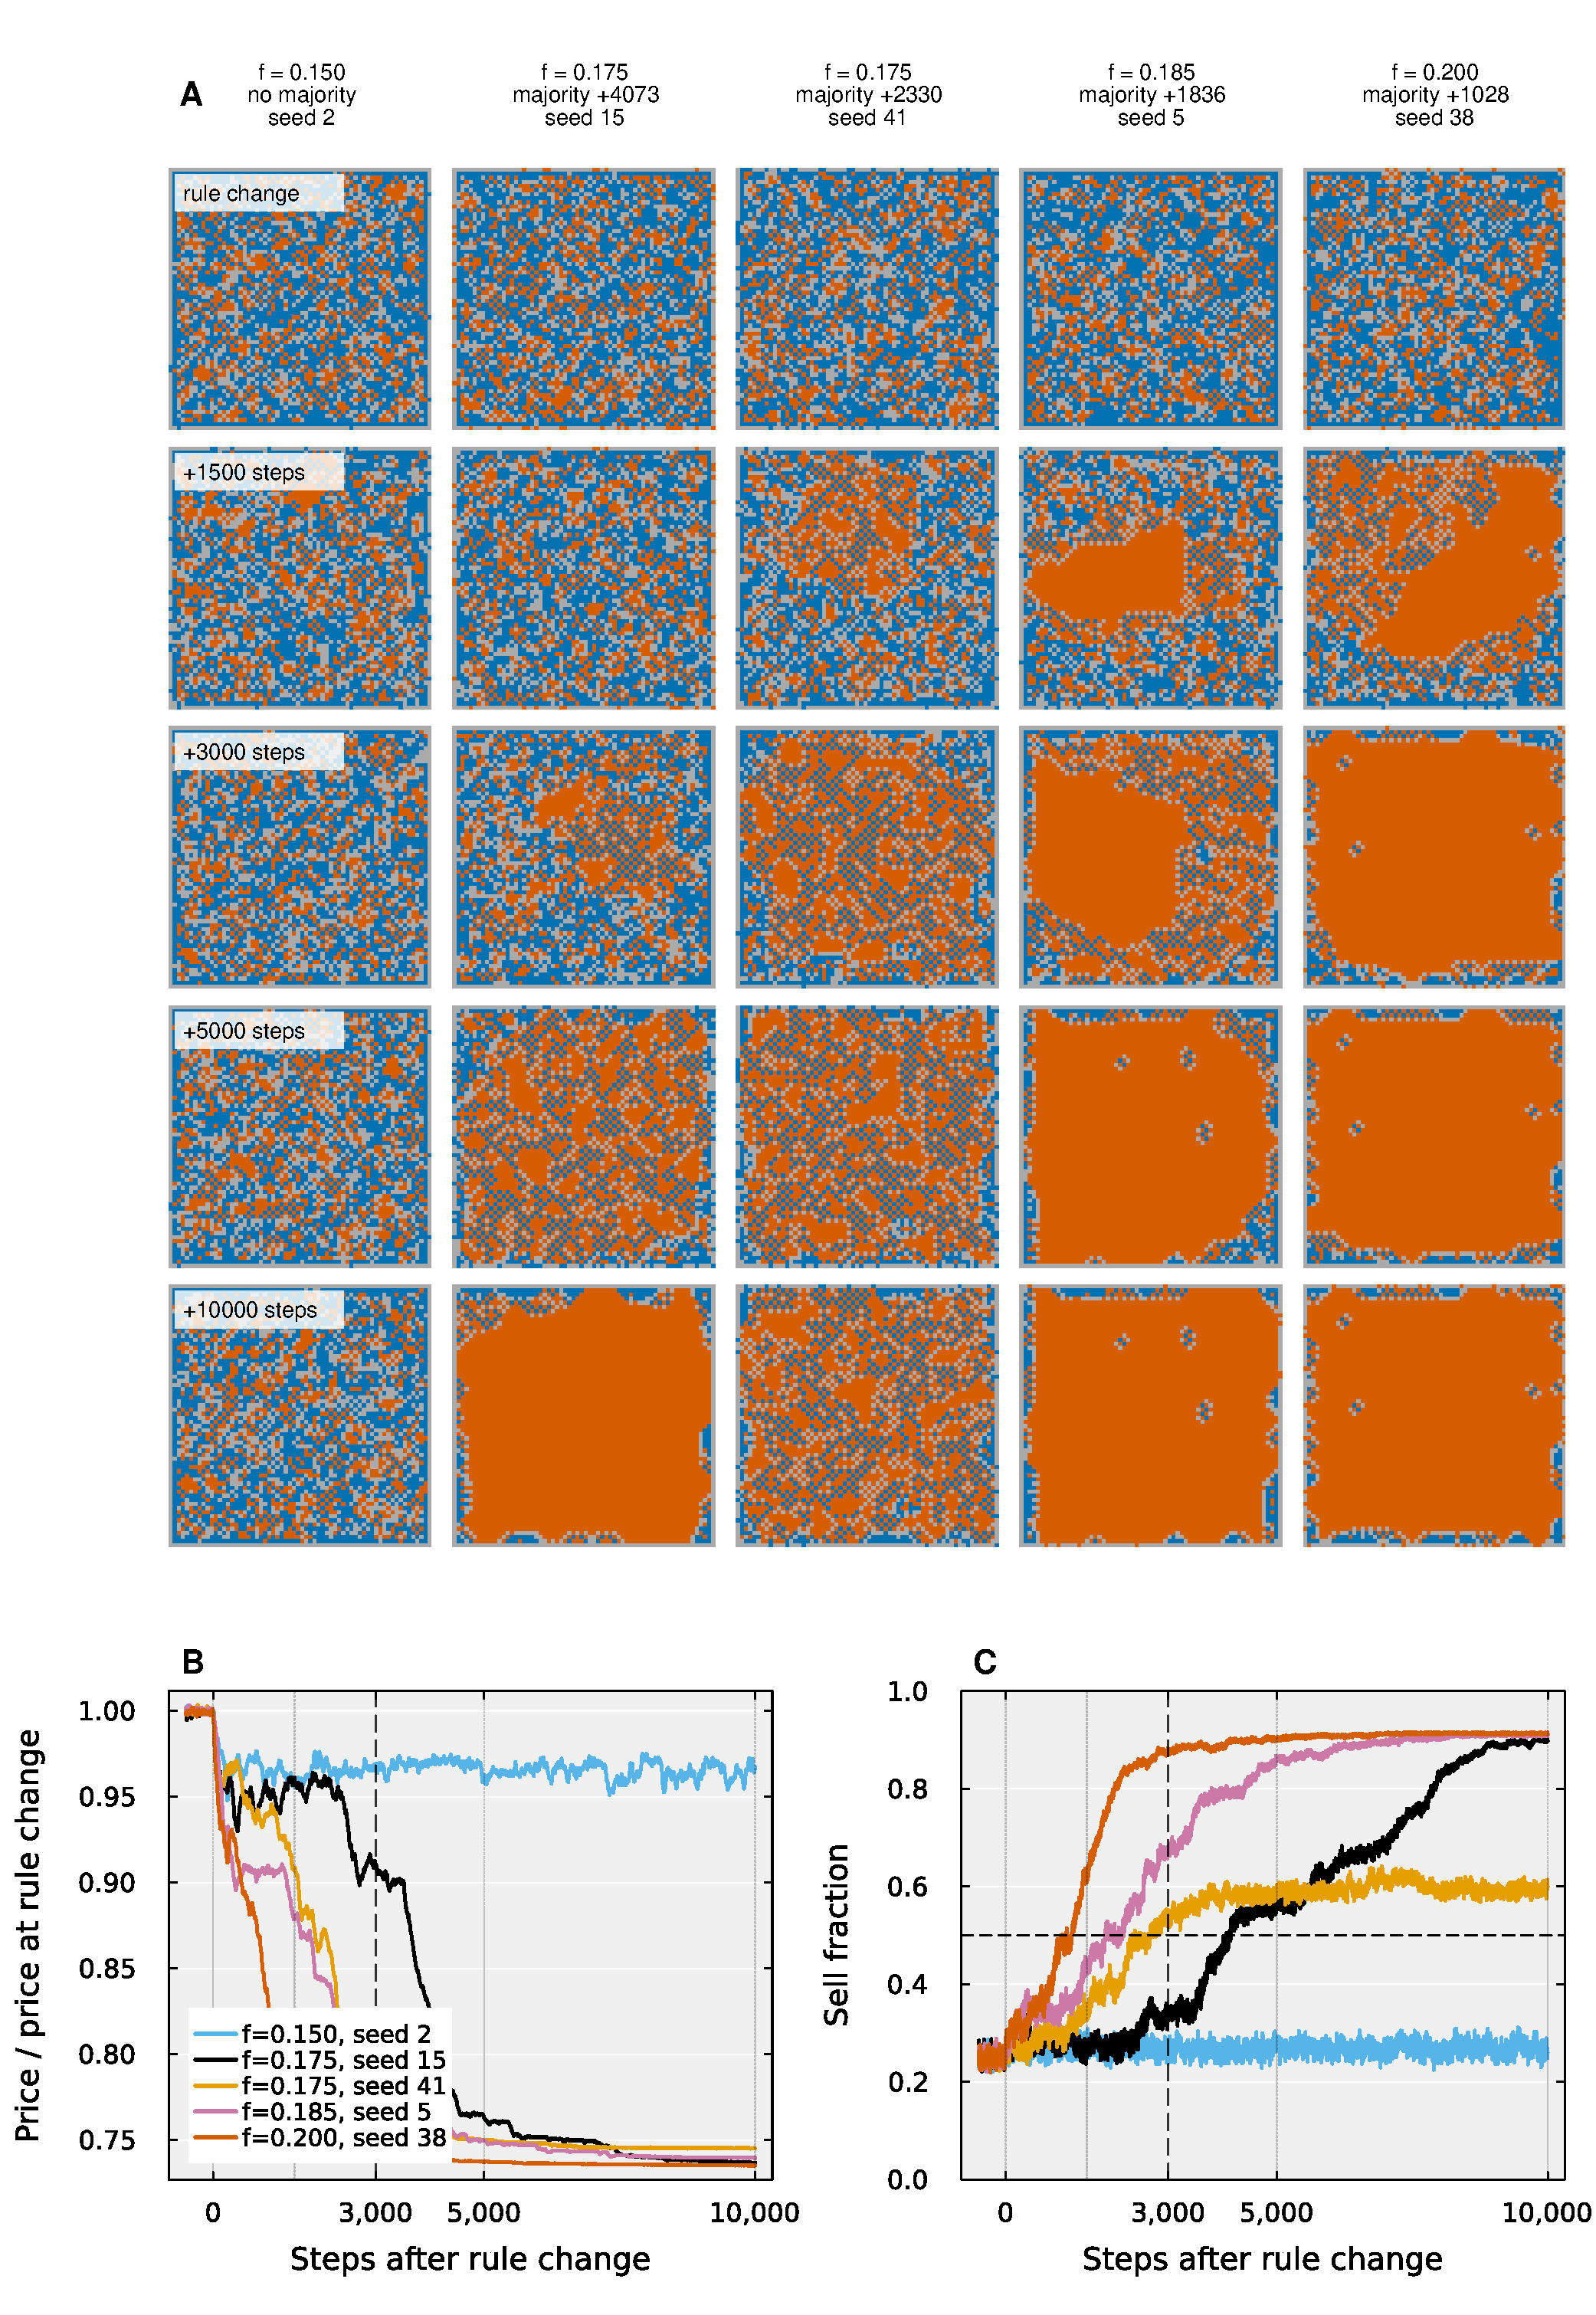
\includegraphics[width=0.90\linewidth]{figs/Fig4-DoseMarketPanels.pdf}
\caption{Longer histories of five numerically selected markets
with active technical traders and $h=100$. Blue, gray, and orange denote
Buy, Hold, and Sell. \textbf{(A)}~Grid decisions at activation and after
1,500, 3,000, 5,000, and 10,000 steps. Selection used the newly computed
3,000-step summaries before inspection of images. At that endpoint,
the first two markets had not reached a majority and the other three
had. Nonmajority examples were nearest their group's median final Sell
fraction; majority examples were nearest their group's median onset,
with seed breaking ties. Starting markets were 2, 15, 41, 5, and 38, from left
to right. The longer outcomes did not affect selection.
\textbf{(B)}~Marginal quote divided by its value at activation.
\textbf{(C)}~Interior Sell fraction, with one-half marked by a
horizontal line. The dark vertical dashed line marks the original
3,000-step endpoint; other guides mark the remaining snapshots.
Onsets and financial summaries appear in Supplementary
Table~\ref{tab:market-panel-horizons}.}
\label{fig:dose-panels}
\end{minipage}
\end{center}

\clearpage

\begin{center}
\begin{minipage}{\linewidth}
\captionsetup{type=figure,hypcap=false}
\centering
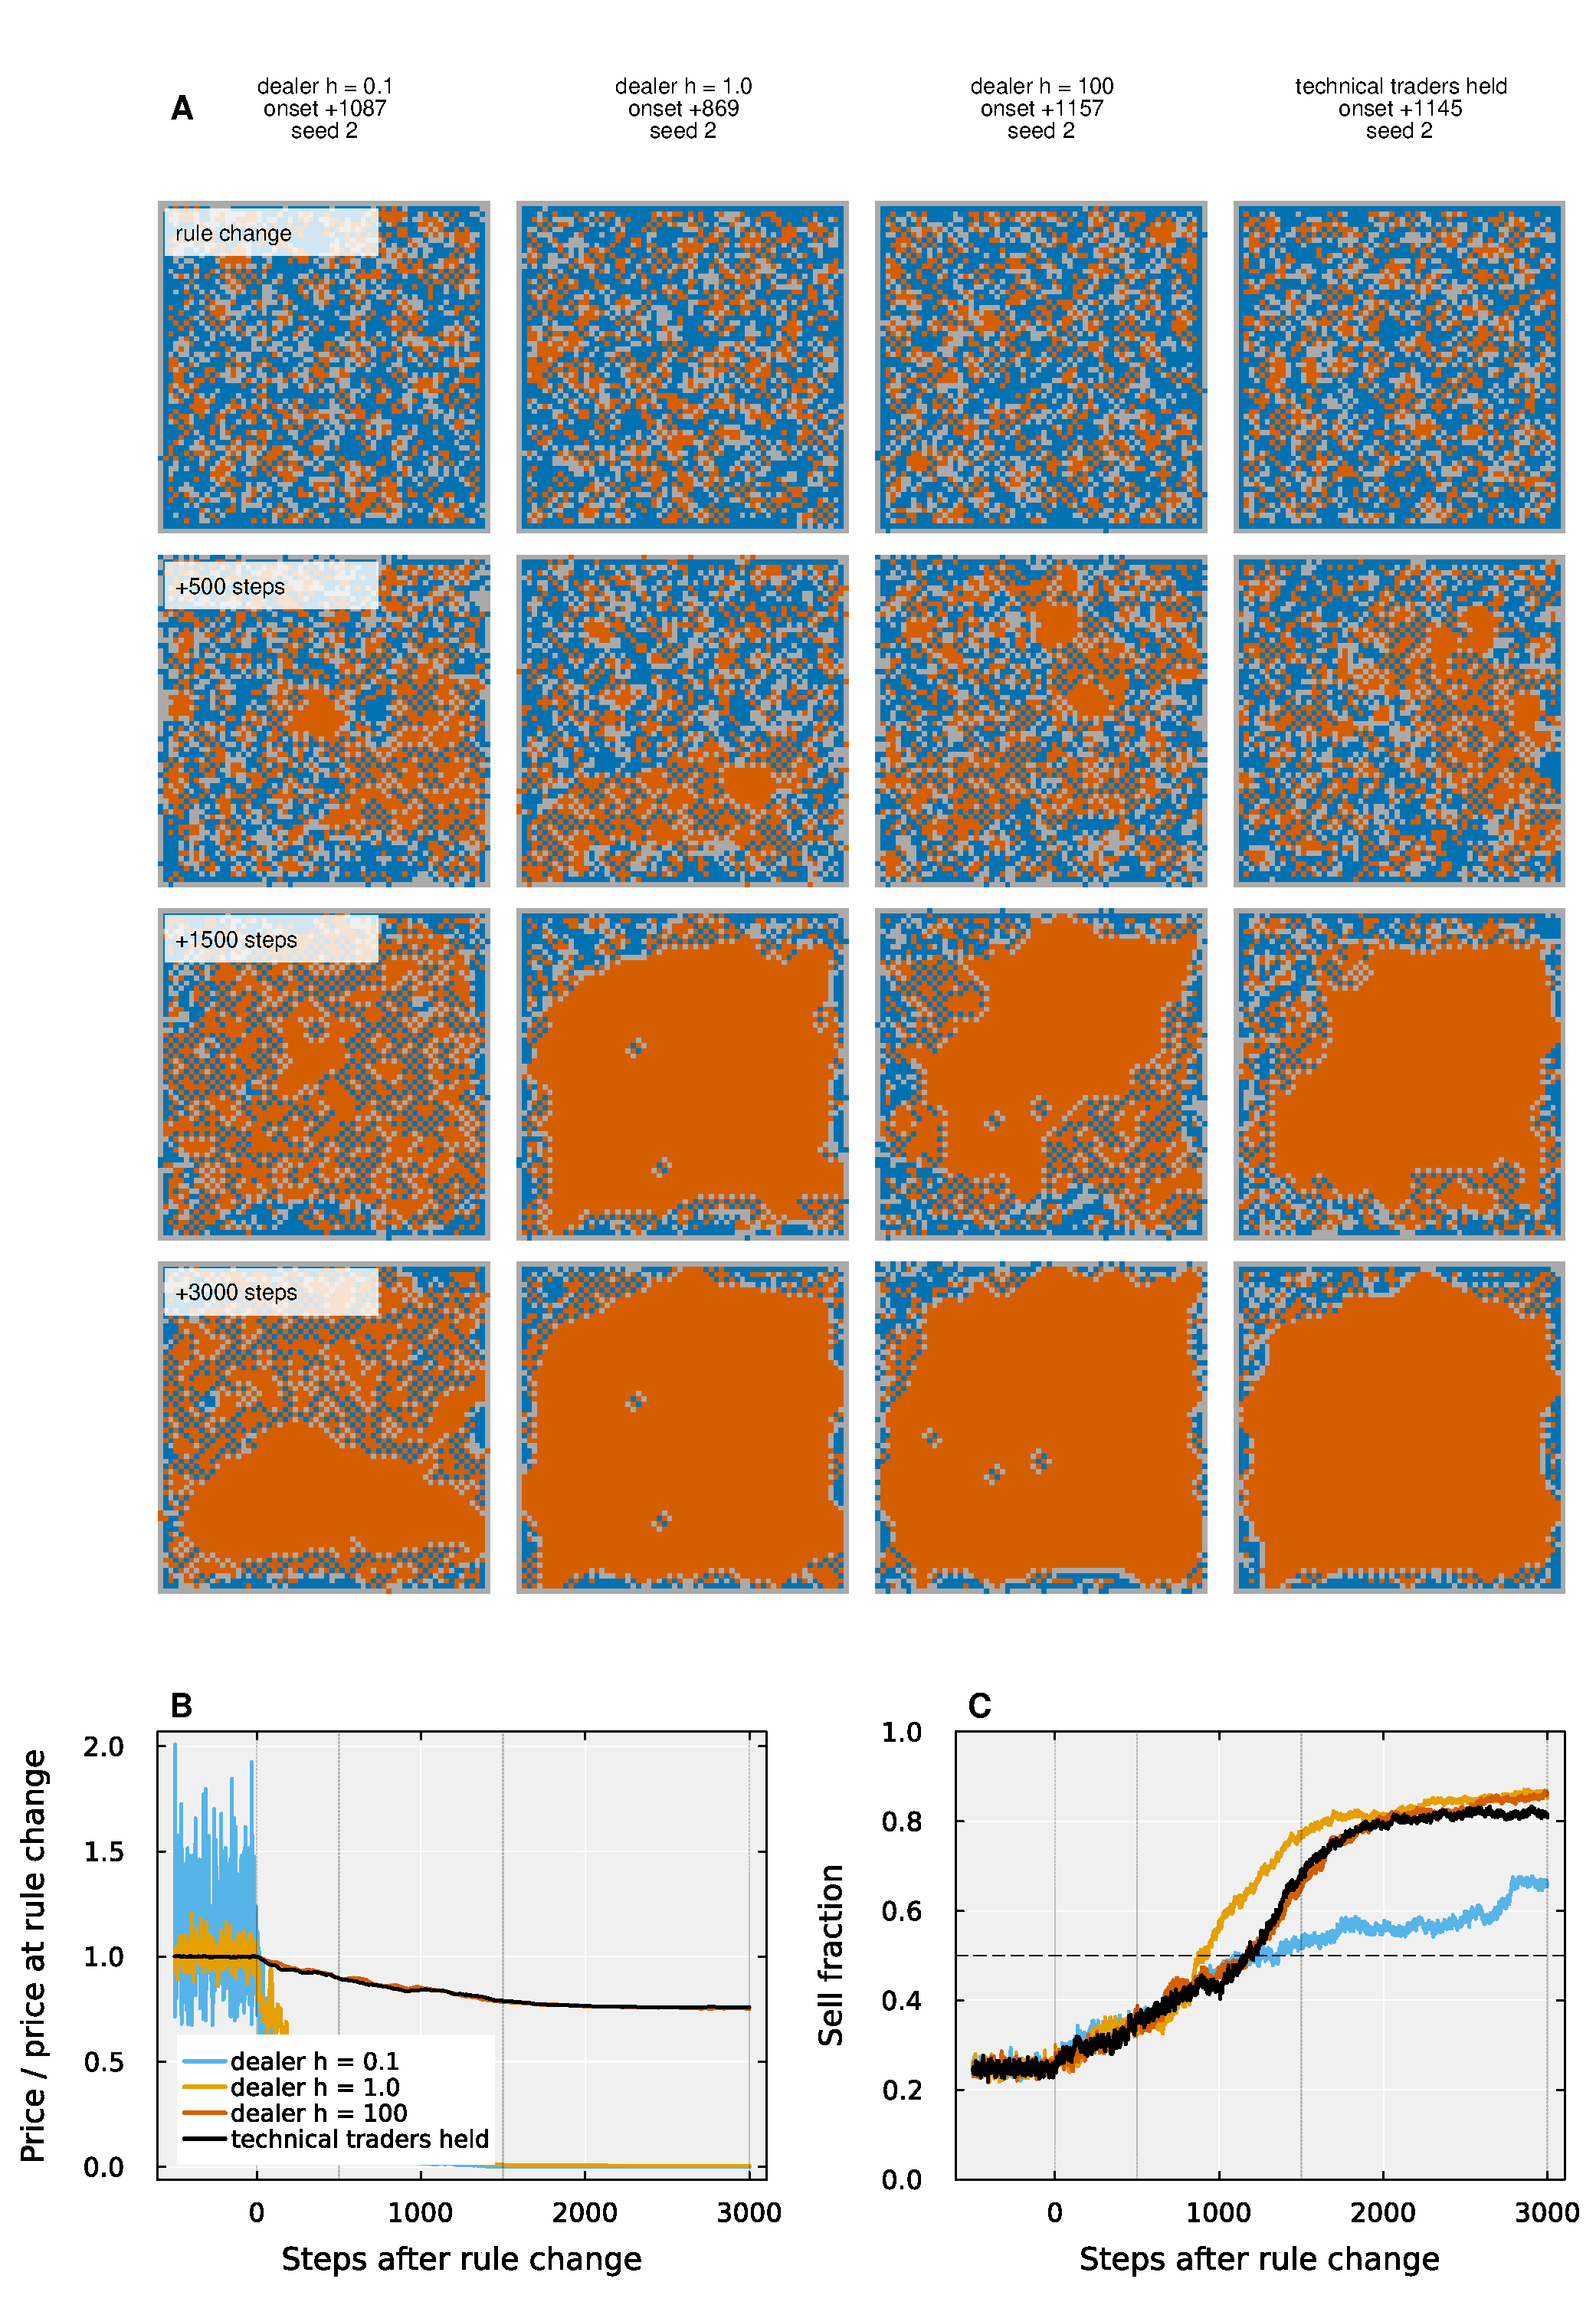
\includegraphics[width=0.92\linewidth]{figs/Fig5-DealerMarketPanels.pdf}
\caption{The same starting market at different dealer depths
with $f=0.20$. \textbf{(A)}~Grid decisions at activation and after
500, 1,500, and 3,000 steps. The first three columns have active technical
traders at $h=0.1$, $1$, and $100$; the last holds the technical traders
at $h=100$. Starting market 2 was selected among
markets reaching a majority at all three active depths by minimizing
the summed distance from their depth-specific median onsets, with seed
breaking ties. \textbf{(B)}~Marginal quote relative to activation.
\textbf{(C)}~Interior Sell fraction. The held condition prevents price
feedback into decisions while retaining full trading and price
calculations. The selected paths illustrate the same initialization
across conditions; ensemble probabilities and drawdowns appear in
Fig.~\ref{fig:reservoir}.}
\label{fig:dealer-panels}
\end{minipage}
\end{center}

\clearpage

\begin{center}
\begin{minipage}{\linewidth}
\captionsetup{type=figure,hypcap=false}
\centering
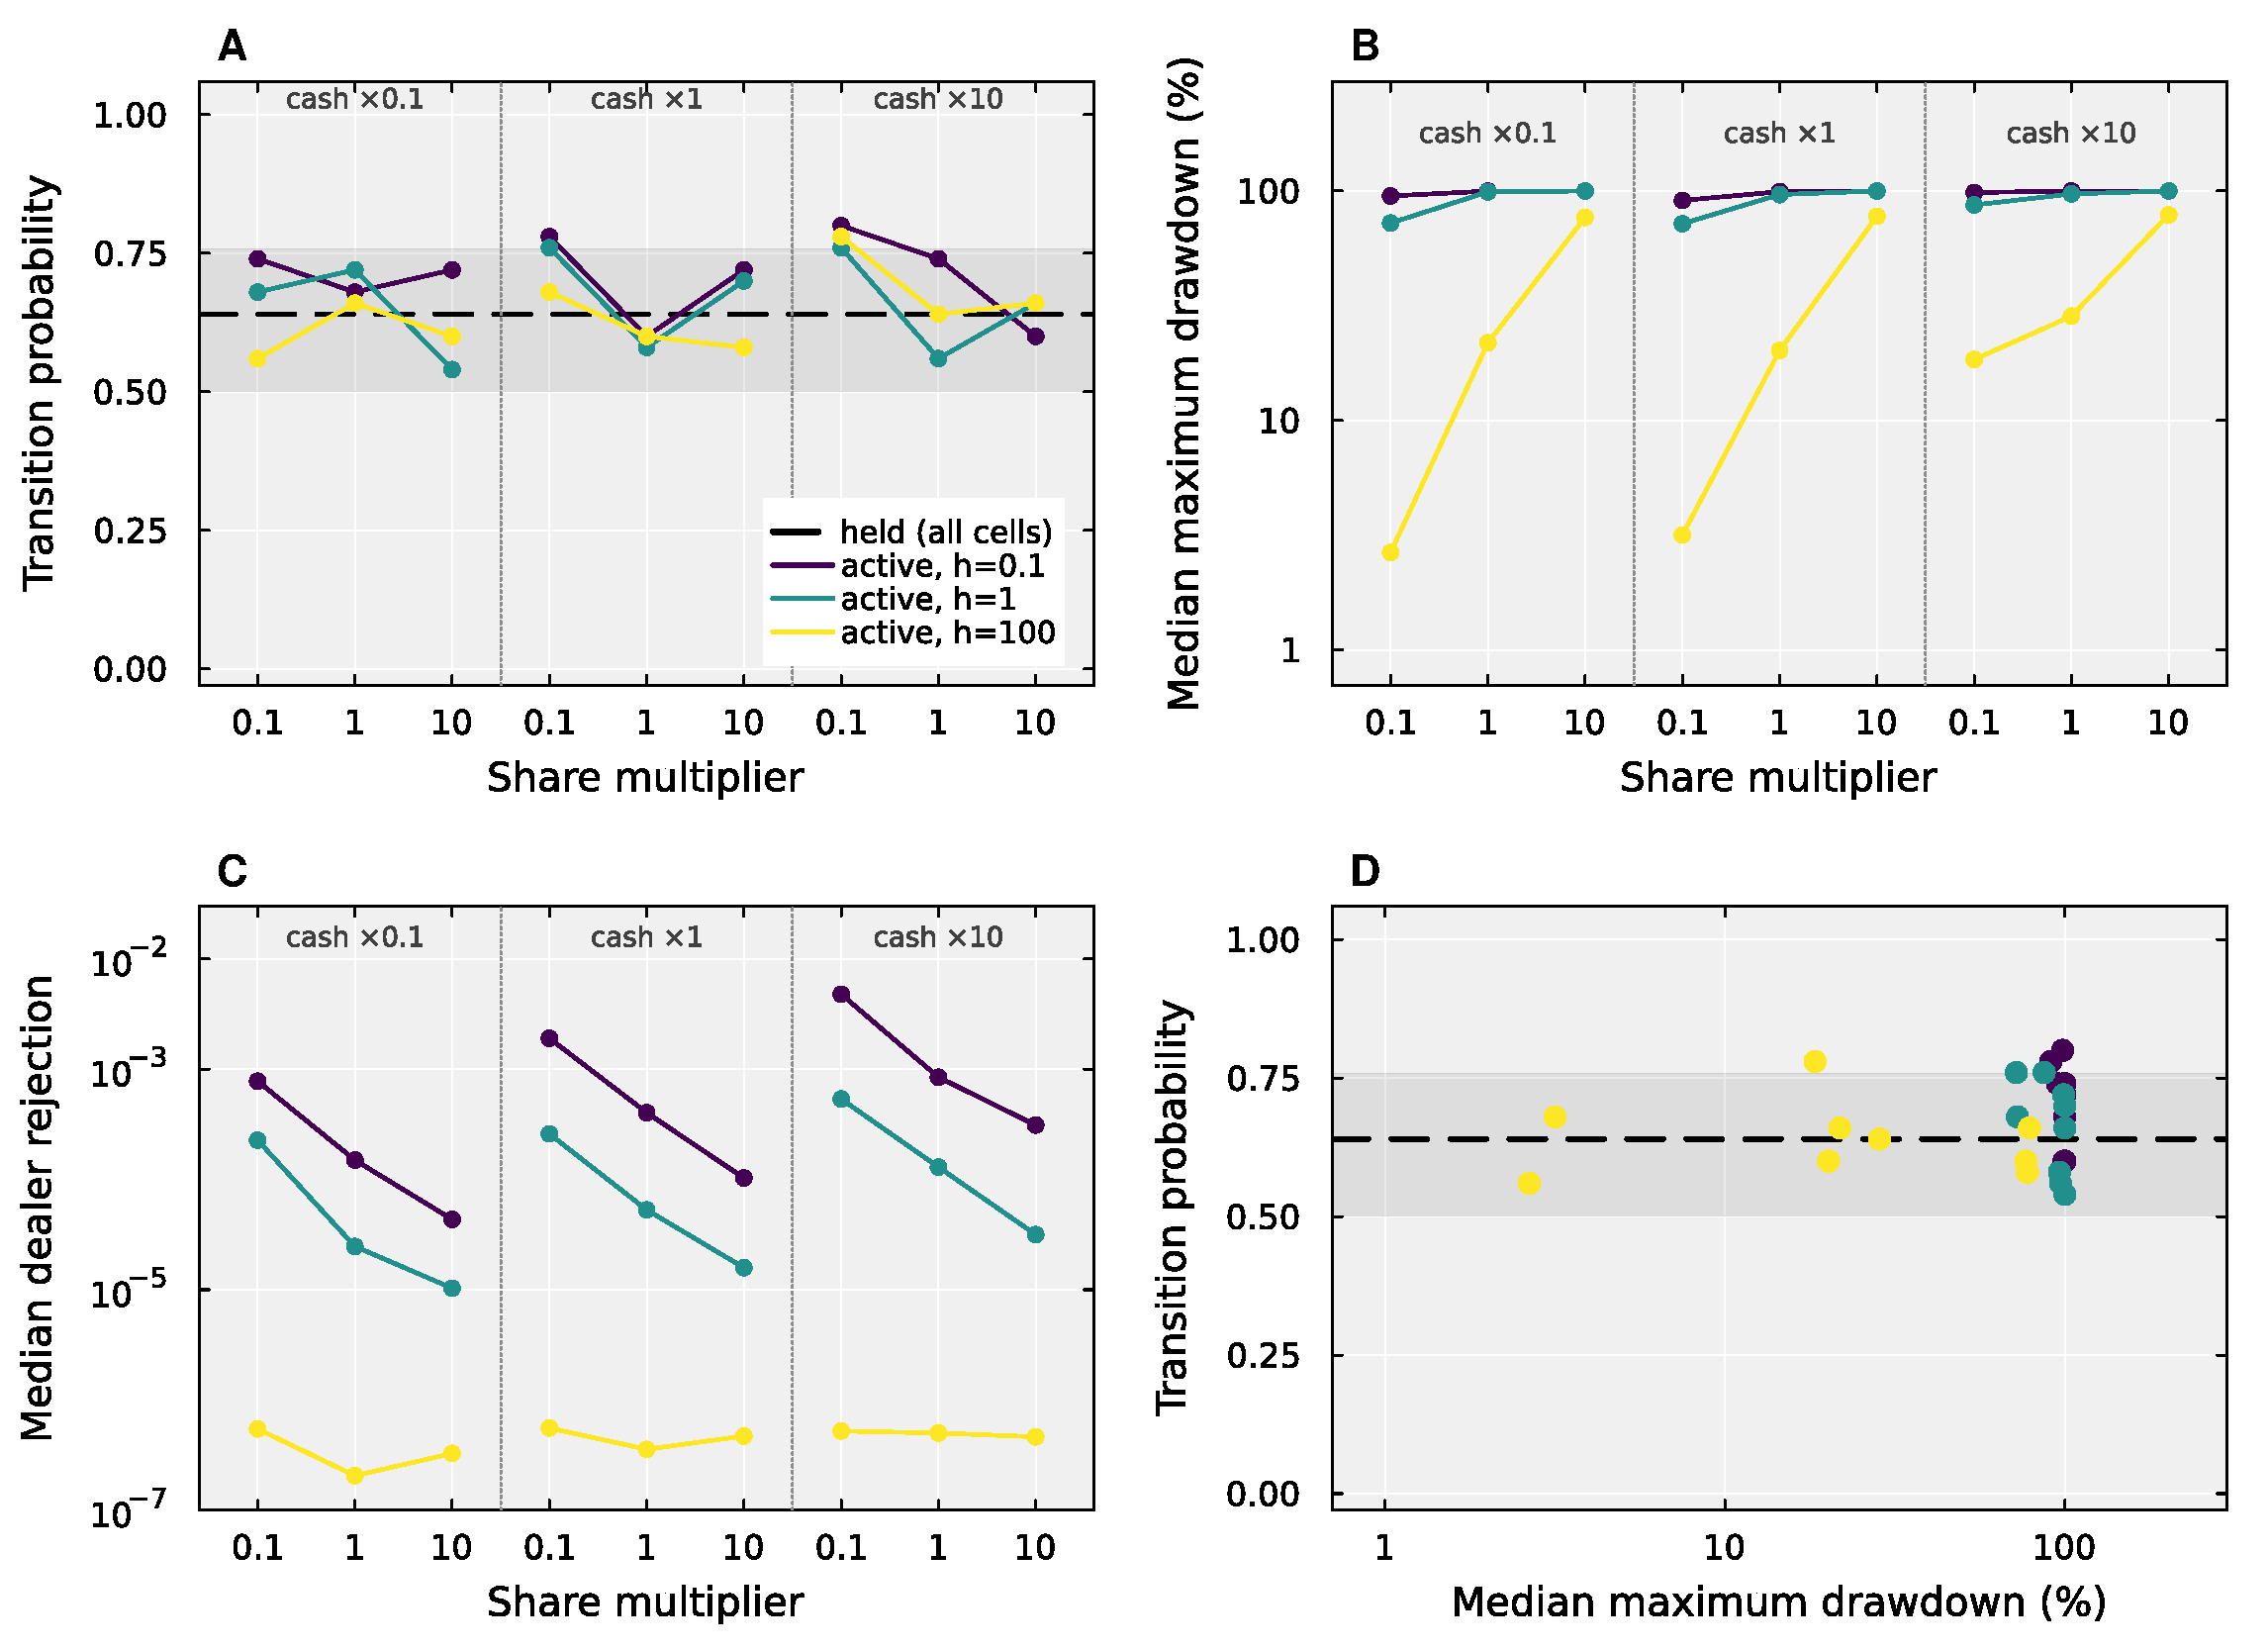
\includegraphics[width=0.99\linewidth]{figs/Fig6-BalanceSheetQuench.pdf}
\caption{Changing trader cash and shares at the rule switch,
with active technical traders, $f=0.18$, and 50 starting markets over 3,000 post-switch steps.
In A--C, the nine resource combinations are grouped by cash multiplier,
with share multiplier on the axis and a series for each dealer depth.
\textbf{(A)}~Majority probability. The dashed line and band give the
held-condition probability and its 95\% Wilson interval, identical
across financial conditions. \textbf{(B)}~Median maximum drawdown on a
logarithmic axis.
\textbf{(C)}~Median fraction of post-switch eligible orders rejected,
on a logarithmic axis.
\textbf{(D)}~Majority probability against median drawdown for all
27 active combinations, with the held reference repeated. The drawdown
axis follows B. Probability axes cover the full possible range;
all displayed drawdowns and rejection medians are strictly positive.}
\label{fig:balance-sheet}
\end{minipage}
\end{center}
